\documentclass[a4paper, 11pt]{article}

\usepackage[danish]{babel}
\usepackage[utf8]{inputenc}
\usepackage{macros}
%\usepackage{tgtermes}
%\usepackage{fouriernc}
\usepackage[T1]{fontenc}
\usepackage[margin=2cm]{geometry}
\usepackage{comment}

\usepackage{graphicx}
\usepackage{amssymb}
\usepackage{gensymb}
\usepackage{amsmath}
\usepackage{amsthm}
\usepackage{multicol}
\usepackage{xcolor}
\usepackage{wrapfig}
\usepackage{array} %skema
\usepackage{subfig} %figurer

\usepackage{enumerate}
\usepackage[shortlabels]{enumitem}
\usepackage{verbatim}
%\usepackage{hyperref}
%\hypersetup{
%    colorlinks=true,
%    linkcolor=red,   
%    urlcolor=red,
%}
\newcommand{\N}{\mathbb{N}}
\newcommand{\Z}{\mathbb{Z}}
\newcommand{\Q}{\mathbb{Q}}
\newcommand{\R}{\mathbb{R}}

%Is defined to be equal to
\newcommand*{\defeq}{\mathrel{\vcenter{\baselineskip0.5ex \lineskiplimit0pt
                     \hbox{\scriptsize.}\hbox{\scriptsize.}}}%
                     =}
 
\title{{\large \textsc{HYDRODYNAMIK\\fysik eksamensprojekt}}}
\author{Cecilie Horshauge}
\date{\today}

\begin{document}
\maketitle
\clearpage
\tableofcontents
\clearpage
\section{Indledning}
Fysikken bag hydrodynamikken er vigtig for flere grene, heriblandt ingengiørfaget og biologi.
Det er fysik som denne, der forårsager at flyvemaskiner kan flyve. Viden om emnet er afgørende for at 
kunne forstå flere biologiske processer og meget mere.\\
Centralt er det, at viden om hydrodynamik har en bred vifte af anvendelser. 
Denne viden muliggører teknologiske og sundhedsmæssige fremskridt og derfor relevant i dag!
I prokjektet vil flere koncepter i hydrodynamikken blive forklaret og disse udnyttes til at udlede 
en matematisk model for tømning af en beholder. 

\clearpage
\section{Formål}
Projektets formål er at stifte bekendtskab med fysikken bag hydrodynamikken. 
Der vil blive præsenteret nye fagbegreber som \textit{laminar} og \textit{turbulent} strømning mf. 
Bernoullis lov og Kontinuitetsligningen gennemgås og udnyttes til at forudsige forløbet af vandspejlets højde ved tømning af en beholder.
\section{Teori}
\subsection{Strømning i væsker}
Væskestrømninger opdeles overordnet set i to grupper: Turbulent og laminar strømning.\footnote{Hansen, O. W. 2008}
En turbulent strømning betyder at strømningen indeholder strømhvirvler, en strømning der ikke har det kaldes laminar.
Derudover siger vi, at en strømning er stationær, hvis hastigheden af en vilkårlig væskepartikel på et givent sted altid har samme retning og størrelse.
\myfigure{0.4}{Images/stromning.png}{Strømningslinjer}{Strømning}\\
På figur \ref*{fig:Strømning} ses et rør med indtegnede strømningslinjer i. Der antages om væsken i røret, at den er inkompressibel, 
dvs. at densiteten \(\rho\) er ens overalt, hvilket gælder for væsker, men ikke for gasser.
Der er vist to tværsnit, \(A_1\) og \(A_2\), på figuren. På grund af rørets tykkelse vil væsken bevæge sig hurtigere ved \(A_2\) end ved \(A_1\).\\\\
Der ses på situationen hvor i tidsrummet \(dt\) strømmer væsken afstanden \(ds_1\) ved \(A_1\) gennem røret og ligeledes stykket \(ds_2\) ved \(A_2\).\\
Betragt nu disse udtryk for væskerumfangene.
\begin{center}
    \begin{tabular}{ l c l }
     \(dV_1=A_1ds_1\) & & \(dV_2=A_2ds_2\)
    \end{tabular}
\end{center}
Derudover er de to rumfang med sikkerhed ens, eftersom væsken er inkompressibel. Vi får da: \(V_1 = V_2\). Strækningen \(ds_1\) og \(ds_2\) kan også defineres ud fra hastigheden og tiden ved:
\begin{center}
    \begin{tabular}{ l c c l }
     \(ds_1=v_1dt\) & & & \(ds_2=v_2dt\)
    \end{tabular}
\end{center}
Derfor kan vi skrive
\[A_1v_1dt = A_2v_2dt\]
\begin{equation}
    A_1v_1=A_2v_2
\end{equation}
\subsection{Bernoullis lov}
Bernoullis lov beskriver sammenhængen mellem trykket \(p\) i et punkt af væsken med strømningshastigheden \(v\) i punktet. \footnote{Young. H. D. side 406-407}
\myfigure{0.4}{Images/bernoulli.png}{Strømning gennem rør med ændrende tværsnit}{Bernoulli}\\
Betragt figur \ref*{fig:Bernoulli}. Vi ser igen på situationen hvor der er strømningslinjer i et rør. På tiden \(dt\) strømmer væsken fra \((a)\) til \((b)\) 
og ligeledes fra \((c)\) til \((d)\). Størrelserne ved forskubningen fra \((a)\) til \((b)\) indekseres med 1 og  forskubningen fra \((c)\) til \((d)\) indekseres med 2.
Det samlede arbejde udført på væsken kan skrives ved: \(dW=F_1ds_1-F_2ds_2\), da \(F=pA\) fås:
\begin{equation}
    \label{eq: 2}
    dW=p_1A_1ds_1-p_2A_2ds_2=p_1dV_1-p_2dV_2.
\end{equation}
Hvis væsken er inkompressibel så gælder der, at \(dV_1=dV_2\).\\
Under forudsætningen at der kan ses bort fra viskositet (gnidning), der gælder
\[\text{Udført arbejde} = \text{tilvækst i energi}\]
\begin{equation}
    \label{eq: 3}
    dW=dE_{kin}+dE_{pot}
\end{equation}
Eftersom strømningen er stationær er den kinetiske energi for væsken mellem \((b)\) og \((c)\) altid den samme.
Tilvæksten i den kinetiske energi er af den grund forskellen mellem de kinetiske energier af væsken ved \(V_1\) og \(V_2\).
\[dE_{kin}=\frac{1}{2}(dm_2)v_2^2-\frac{1}{2}(dm_1)v_1^2\;,\;\;\; \text{hvor } dm_1=dm_2=\rho dV\]
Derfor kan vi skrive
\begin{equation}
    \label{eq: 4}
    dE_{kin}=\frac{1}{2}\rho v_2^2 dV-\frac{1}{2}\rho v_1^2 dV
\end{equation}
Den potentielle energi kan regnes ved \(E_{pot}=mgy\), hvor y betegner afstanden over jorden. Tilvæksten i den potentielle energi kan derfor skrives ved
\begin{equation}
    \label{eq: 5}
    dE_{pot}=(dm_2)gy_2-(dm_1)gy_1 = \rho g y_2 dV-\rho g y_1 dV
\end{equation}
Ved indsættelse af ligning \ref*{eq: 2}, \ref*{eq: 4} og \ref*{eq: 5} i ligning \ref{eq: 3} fås:
\[p_1dV-p_2dV=\underbrace{\;\frac{1}{2}\rho v_2^2dV - \frac{1}{2} \rho v_1^2dV}_{dE_{kin}} + \underbrace{\rho g y_2 dV - \rho g y_1 dV}_{dE_{pot}}\]
Vi kan nu forkorte \(dV\) væk og omrorkere leddene.
\begin{equation}
    \label{eq: Bernoullis}
    p_1+\frac{1}{2} \rho v_1^2+\rho g y_1 = p_2+\frac{1}{2} \rho v_2^2+\rho gy_2
\end{equation}
Vi har u udledt Bernoullis lov.
\subsection{Kontinuitetsligningen}
Massen af en væske med en konstant strømning ændrer sig ikke. \footnote{Young. H. D. side 404-405}
Dette leder til et resultat kendt som Kontinuitetsligningen. Betragt to dele af en gennemstrømningsrør med strømning mellem to tværsnit, \(A_1\) og \(A_2\).Vi kan igen betragte figur \ref{fig:Bernoulli}.
Kald hastighederne af væskerne ved tværsnitene for henholdsvis \(v_1\) og \(v_2\).
Der flyder ikke væske ud af siderne af strømningsrøret og heller ikke ind af det. 
På den korte tid \(dt\), bevæger væsken ved \(A_1\) sig afstanden \(ds_1=v_1 dt\). En cylinder med højden \(v_1\) og grundfladen \(A_1\) vil have volumen \(dV_1=A_1 v_1 dt\). 
Dette volumen er hvad der strømmer forbi \(A_1\) i tidsrummet \(dt\). Ligeledes (i samme tidsrum \(dt\)) for en cylinder med volumen \(dV_2=A_2v_2 dt\) strømmer i gennem \(A_2\).\\
Først antages der at væsken er inkompressibel, dvs. at massefylden er den samme overalt. Massen der passerer gennem \(A_1\) i tiden \(dt\) må være \(dm_1=\rho A_1 v_1 dt\) og det samme gælder for sektion 2: \(dm_2=\rho A_2 v_2 dt\). 
Under en stationær strømning er massen tilsammen i røret konstant, vi får da \(dm_1=d_2\) og dermed også 
\[\rho A_1 v_1 dt= \rho A_2 v_2 dt\]
Og der fås kontinuitetsligningen for en inkompressibel væske
\begin{equation}
    A_1 v_1 = A_2 v_2
\end{equation}
hvor \(A_1\) og \(A_2\) er tværsnittet af et strømningsrør ved to steder. Desuden er \(v_1\) og \(v_2\) strømningshastigheden ved de to steder. 
\section{Fremgangsmåde}
En cylinder med et mindre hul i bunden fyldes med vand. Hullet skal dækkes til indtil man har fyldt cylinderen med en tilpasmængde vand - ca. så vandstanden er 80 cm over bunden af cylinderen.
Man lader vandet løbe ud af bunden og filmer opstillingen lige på. Dataene behandles i LoggerPro. Forsøgsopstillingen kan ses på bilag 1.
\section{Forventninger for forsøget}
Vi siger at højden \(h\) er afstanden fra vandspejlet til bunden af cylinderen. Væsken har massefylden \(\rho\). Vi kan opskrive situationen med Bernoullis ligning, her udelades leddet med trykket under antagelse at trykket på vandspejlet og i bunden af cylinderen er det samme.
\begin{equation}
    \frac{1}{2}\rho v_1^2+\rho g h_1 = \frac{1}{2}\rho v_2^2+\rho g h_2
\end{equation}
hvor der gælder at ved \(h=0\) er \(v=0\) og ved dybden \(h\) er hastigheden \(v\).
Her kan det ses at Bernoullis lov giver det samme som gælder for frit fald i tyngdefeltet.
\begin{equation}
    \frac{1}{2}\rho v^2+\rho g (-h)=0 \Leftrightarrow v=\sqrt{2gh}
\end{equation}
Hastigheden \(v\) betegner den hastighed væsken løber ud af bunden med. 
Vi kalder funktionen \(m(t)\) for massen af væsken som funktion af tiden. Vi siger at bundens åbning har tværsnitsarealet \(D\).
For denne sammenhæng må kontinuitetsligningen gælde hvor \(dm\) er ændringen af væskens masse i tidsrummet \(dt\) som vandet strømmer ud af cylinderen.
\[\frac{dm}{dt}=-\rho Dv\]
Hvis vi kalder cylinderens tværsnit for \(A\), så kan massen regnes ved \(m=\rho A h\), hvilket medfører
\[\frac{dm}{dt}= \rho A \frac{dh}{dt}\]
Vi kan sætte de to udtryk lig med hinanden, vi får
\[pA \frac{dh}{dt}=-\rho Dv\]
hvis der derudover indsættes \(v=\sqrt{2gh}\) fra før, fås følgende differentialligning
\begin{equation}
    \rho A \frac{dh}{dt} = -\rho D \sqrt{2gh} \Leftrightarrow \frac{dh}{dt} = -\sqrt{2g}\, \frac{D}{A}\sqrt{h} 
\end{equation}
Vi løser differentialligningen ved separation af variable og integration
\begin{align*}
    \frac{dh}{\sqrt{h}}&=-\sqrt{2g}\,\frac{D}{A}dt\\
    \int_{h_0}^{h}\frac{dh}{\sqrt{h}}&=-\sqrt{2g}\,\frac{D}{A} \int_0^t dt\\
    2\sqrt{h}-2\sqrt{h_0}&=-\sqrt{2g}\frac{D}{2A}t\\
    h&=\left(\sqrt{h_0}-\frac{D\sqrt{2g}}{2A}t\right)^2
\end{align*} 
Vi forventer altså at højden som funktion af tiden følger overstående udvikling ved tømning af en beholder.
\section{Hypotese}
Der forventes at ved tømning af en beholder med tværsnitsareal A og tværsnitsarealet D af beholderens åbning og begyndelseshøjde \(h_0\). Der vil vandstandens højde \(h\) som funktion af tiden \(t\) følge udviklingen
\begin{equation}
    h=\left(\sqrt{h_0}-\frac{D\sqrt{2g}}{2A}t\right)^2
\end{equation}
på baggrund af ovenstående teori.
\clearpage
\section{Analyse og resultater}
Forsøget er blevet repeteret af flere omgange. Ved hver figur \((a)\) kan man se dataene plottet sammen med de forventede værdier for hver repetition af forsøget. Ved hver figur \((b)\) ses et residualplot af dataene i henhold til de forventede data.\\
Her ses graferne for 3 repetitioner af forsøget med et 5 mm i diameter hul i bunden.
\begin{figure}[!h]%
    \centering
    \subfloat[\centering Data plottet sammen med forventning]{{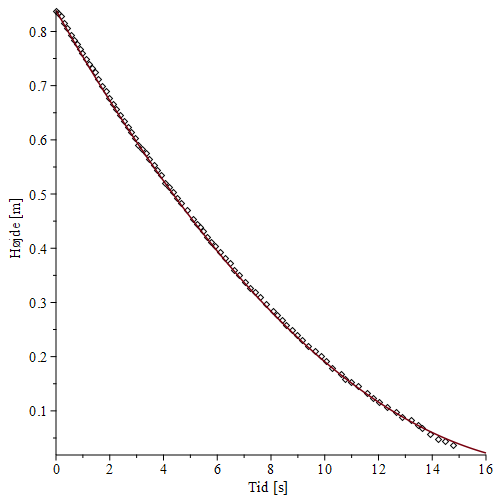
\includegraphics[width=6.8cm]{Images/plot4.png} }}%
    \quad
    \subfloat[\centering Residualplot for forsøget]{{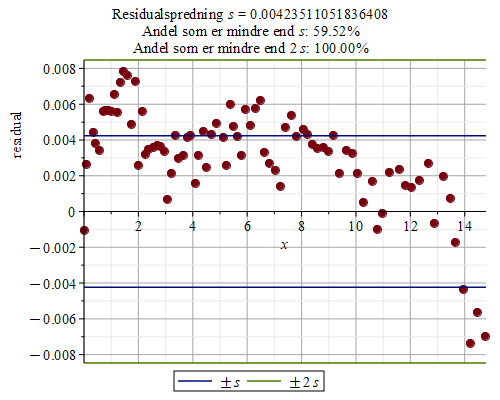
\includegraphics[width=8.5cm]{Images/residualPlot4.png} }}%
    \caption{Resultater for forsøg 1}%
    \label{fig:resultat1}%
\end{figure}\\
\begin{figure}[!h]%
    \centering
    \subfloat[\centering Data plottet sammen med forventning]{{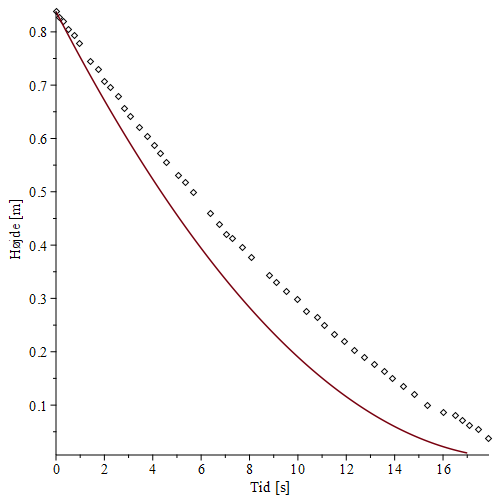
\includegraphics[width=6.8cm]{Images/plot5.png} }}%
    \quad
    \subfloat[\centering Residualplot for forsøget]{{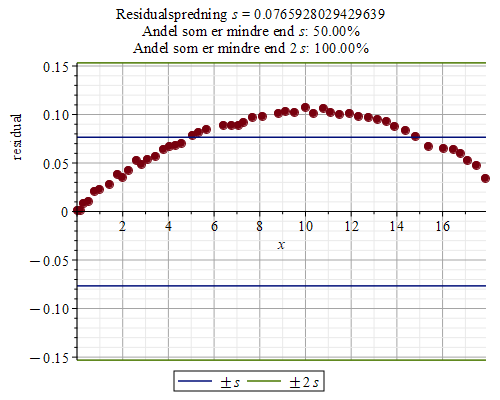
\includegraphics[width=8.5cm]{Images/residualPlot5.png} }}%
    \caption{Resultater for forsøg 2}%
    \label{fig:resultat2}%
\end{figure}\\
\begin{figure}[!h]%
    \centering
    \subfloat[\centering Data plottet sammen med forventning]{{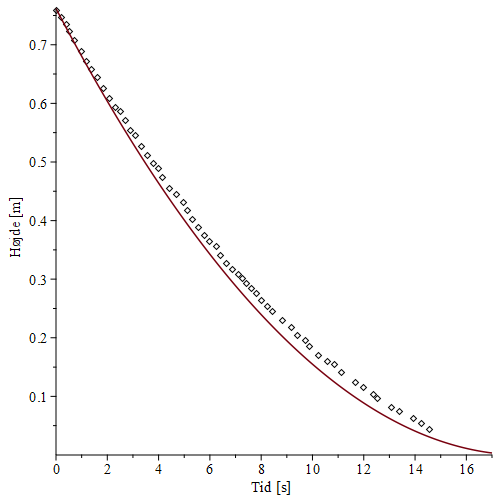
\includegraphics[width=6.8cm]{Images/plot6.png} }}%
    \quad
    \subfloat[\centering Residualplot for forsøget]{{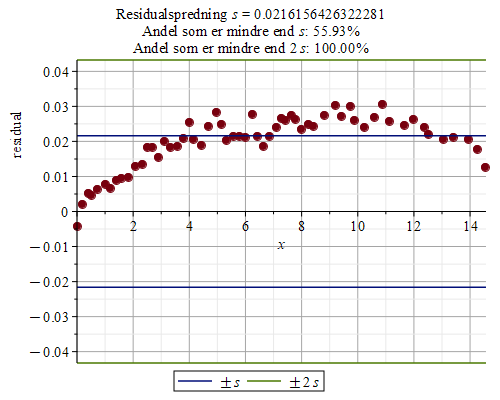
\includegraphics[width=8.5cm]{Images/residualPlot6.png} }}%
    \caption{Resultater for forsøg 3}%
    \label{fig:resultat3}%
\end{figure}
\newpage
\section{Diskussion}
Graferne viser dataene plottet med den forventede tømning af cylinderen. På figur \ref*{fig:resultat1} \((a)\) kan man se at dataene følger den matematiske model meget pænt. 
Ved \((b)\) kan man se at den beregnede residualspredning for forsøget er udregnet til \(s_1=0.000424\) - altså en temmelig lille spredning. \footnote{Gennemsnitlig kvadratafvigelse}
Hele datasættet ligger indenfor 2 residualspredninger og \(59.52\%\) ligger inden for 1 spredning. Det vil sige at dataene i forsøg 1 følger modellen temmelig godt.\\\\
Figur \ref*{fig:resultat2} viser resultatet af forsøg 2, på grafen \((a)\) er ses det at alle datapunkterne ligger for højt. På residualplottet \((b)\) er det klart at en større fejlkilde har spillet ind, residualspredningen er mere end end faktor 10 større end forsøg 1, den ligger på \(s_2=0.0770\), altså markant større.\\
Der har været en eller flere systematiske fejlkilder. Her må vi huske at den matematiske model er lavet på baggrund af følgende antagelser:
\begin{enumerate}
    \item Strømningen er laminar
    \item Væsken er viskositetsfri
    \item Væsken er inkompressibel
\end{enumerate}
Man kan se på videoen optaget af forsøg 2 at ved forsøgets start skulle cylinderen lige til at tippe, og når også at tippe lidt, i forbindelse med at den rettes op igen vipper vandspejlet op og ned. 
Det formodes at grunden til forsøg 2 afviger mere end de to andre er pga. denne ændring i strømningen.
Hvis ændringen i strømningen har forårsaget at strømningen er blevet delvist turbulent fremfor laminar, så er det en selvfølge at observationerne ikke vil følge den laminare model.\\\\
% 3
Ved forsøg 3 kan vi se på figur \ref*{fig:resultat3} \((a)\) at dataene tilnærmelsesvist følger udviklingen. Men at der igen er en systematisk fejlkilde. Dette ses klarere ved \((b)\) residualplottet over dataene, her er residualspredningen bestemt til \(s_3=0.0216\), altså en lav residualspredning. 
I plottet er alle datapunkter indenfor 2 spredningers afvigelse og \(56.93\%\) ligger inden for 1 spredning.\\\\
% samlet
Det ser desuden også ud til at der har været en systematisk fejlkilde for både forsøg 1 og 3, dog betydelig mindre end for forsøg 2, og derfor sandsynligvis ikke samme fejlkilde.
Den afvigelse vi her ser på figur \ref*{fig:resultat1} og \ref*{fig:resultat3} må skyldes vands viskositet. Vi havde oprindeligt antaget at væsken var viskositetsfri, men det er ikke helt sandt. Vand har en meget lav viskositet, men den er der trodsalt.
Olie eller sirup har for eksempel en betydeligt større viskositet, så vi ville forvente af tømningen af en cylinderfuld af sirup ville tage endnu længere tid. og dermed ville få en meget stor fejlkilde, da modellen under antagelse at væsken er viskositetsfri er den samme.
\begin{comment}
\subsection{Fluid Dynamics}
Her er nogle eksempler på fluid dynamics i virkeligheden
\begin{itemize}
    \item Tornado
    \item Flyvemaskiner, holdt oppe af lufttryk på vingerne
    \item Væske i vores bremser
    \item Vores krop
\end{itemize}
\subsection*{Densitet}
Densitet er masse per volumen og har SI enheden kg/\(\text{m}^3\).
\begin{equation}
    \label{densitet}
    \rho = \frac{m}{V}
\end{equation}
Vands densitet er som regel i nærheden af 1000 kg/\(\text{m}^3\). Hvor lufts densitet er cirka en faktor 1000 mindre.\\
Om væsker siger vi, at de er ikke-komprimerbare, deres densitet er forbliver altså næsten konstant. Gasser derimod kan komprimeres og kaldes derfor for komprimerbare.
\subsection*{Tryk}
I fluid mechanics defineres tryk som kraften en væske udfører per areal. SI enheden er \(\text{N}/\text{m}^2\), som kaldes pascal (Pa).
\begin{equation}
    \label{tryk}
    p=\frac{F}{A}
\end{equation}
Tryk er en skalar. I et givent punkt i en væske, er tryk fordelt ens i alle retninger. Det giver derfor ikke mening at tale om en retning. 
\subsection*{Hydrostatisk ligevægt}
Hydrostatisk ligevægt eller hydrostatisk balance (eng: Hydrostatic equilibrium) er den tilstand hvor summen af alle kræfter der virker på fluiden er lig 0.\\\\
Når der er tyngdekraft tilstede [...]
\subsection*{Pascals lov}
\end{comment}
\section{Perspektivering}
I dette projekt er flere nye begreber og sammenhænge blevet introduceret for at kunne beskrive tømning af en beholder med væske.
Men disse er også med til forklare mange andre sammenhænge i verden.\\
Kontinuitetsligningen forklarer f.eks. hvorfor at hælde honning ud ser ud som det gør og forløber sådan.\footnote{Young. H. D. (2020) side 405}
Når der hældes honning ud af en beholder øges strømningshastigheden i takt med at der hældes. Hastigheden er altså lavere ved beholderens munding end længere nede. 
Det er også derfor at tværsnitsarealet er større ved mundingen end forneden.\\
Bernoullis lov kan desuden også forklare hvorfor en giraf med højt blodtryk er sund og rask.\footnote{Ibid. side 407} 
Som følge af Bernoullis lov må blod der strømmer fra hjertet og op til hjernen have en konstant hastighed. 
Trykket \(p\) vil falde som blodets højde \(y\) forstørres. For at blodet kan nå fra hjertet til menneskers hjerner med det mindst mulige tryk, tilfører hjertet et maximum på 120 mm Hg (systolisk) tryk. 
Den lodrette afstand fra hjerte til hjerne er betydeligt større for en giraf, så en girafs hjerte skal altså levere et betydeligt større tryk - ca. 280 mm Hg.\\
Der er blevet stiftet bekendtskab med laminare strømninger.\footnote{Ibid. side 411} Blodet der strømmer i vores blodårer er en laminar strømning. 
Men selv små forstyrrelser, eksempelvis hjerteforstyrrelser gøre at blodstrømningen turbulent. 
Da turbulens larmer, bruges et stetoskop typisk i forbindelse med diagnostisering.\\
På den måde er kan hydrodynamikken forklare en bred vifte af sammenhænge, disse var kun et par korte nedslag fra virkeligheden.
\section{Konklusion}
Vi har set at man ved hjælp af hydrodynamikkens love kan forudsige forløbet af en beholders tømning. 
Til udledning af forløbet er Bernoullis lov og Kontinuitetsligningen blevet anvendt. Der blev fremstillet en matematisk model 
for den forventede tømning af beholderen, der er som følger:
\[h=\left(\sqrt{h_0}-\frac{D\sqrt{2g}}{2A}t\right)^2\]
Denne udledning er testet ved at tømme en beholder fyldt med vand gentagne og gange. 
Resultaterne viser at tømningen foregår tilnærmelsesvist efter den bestemte model. 
Næsten alle målte højder havde en tendens til at være lidt større end forventet. 
Altså tømningen tog lidt længere tid end forventet. Denne fejlkilde forventes at skyldes vands viskositet, der ikke er taget højde for et i den teoretiske model.\\
\clearpage
\section{Litteraturliste}
\textbf{Primær liste}\\\\
Hansen, O. W. (2008). \textit{Bernoullis lov Med eksempler fra Hydrodynamik og Aerodynamik}.\\\\
Young, H. D. \& Freedman, R. A. (2020). \textit{University Physics with Modern Physics}. Pearson.\\\\
\textbf{Sekundær liste}\\\\
Hansen, O. W. (2012). \textit{Der er hul i spanden}. LMFK-bladet.\\\\
Wolfson, R. (2021). \textit{Essential University Physics Volume 1}. Pearson.
\clearpage
\section{Bilag}
\textbf{Bilag 1}\\\\
\includegraphics[width=0.7 \textwidth]{Images/forsøgsopstilling.png}
\end{document}